\documentclass[11pt]{article}
\usepackage{geometry}                
\geometry{letterpaper}                 
\usepackage[parfill]{parskip}        
\usepackage{graphicx}
\usepackage{amssymb}
\usepackage{amsmath}
\usepackage{epstopdf}
\usepackage{verbatim}
\usepackage{float}
\usepackage{enumerate}
\usepackage{hyperref}
\usepackage[utf8]{inputenc}
\usepackage[T1]{fontenc}
\DeclareGraphicsRule{.tif}{png}{.png}{`convert #1 `dirname #1`/`basename #1 .tif`.png}
\usepackage{color}
\usepackage{textcomp}
\definecolor{listinggray}{gray}{0.9}
\definecolor{lbcolor}{rgb}{1,1,1}

\begin{document}
{\small
\section*{Problems for Discussion 7, 11/06/13}
Compiled by Mai Le
}

\section{Questions about overlap add or overlap-save?}

\section{DSP tricks}
Byron is faced with computing \textbf{lots} of discrete Fourier transforms. He will, of course, use the FFt algorithm, but he is behind schedule and needs to get his results as quickly as possible. He gets the idea of computing \textbf{two} transforms at one time by computing the transform of $s[n]=s_1[n]+j s_2[n]$, where $s_1[n]$ and $s_2[n]$ are two real-valued signals of which he needs to compute the spectra. The issue is whether he can retrieve the individual DFTs from the results or not.

\begin{description}
\item[a)] What will the DFT $S[k]$ of this complex-valued signal in terms of $S_1[k]$ and $S_2[k]$, the DFTs of the original signals?
\item[b)] Byron's friend, an Aggie who knows some signal processing, says that retrieving the wanted DFTs is easy: "Just find the real and imaginary parts of $S[k]$." Show that this approach is too simplistic.
\item[c)] While his friend's idea is not correct, it does not give him an idea. What approach will work? \textbf{Hint}: Use the symmetry properties of the DFT.
\item[d)] How does the number of computations change with this approach? Will Byron's idea ultimately lead to a faster computation of the required DFTs?
\end{description}

{ \color{blue}
\begin{description}
\item[(a)] Form linearity of the DFT, $S[k] = S_1[k]+jS_2[k]$.
\item[(b)] $Re\{S[k]\} = Re\{S_1[k]\} - Im\{S_2[k]\}$ and $Im\{S[k] = Im\{S_1[k]+Re\{S_2[k]\}$. Because $S_1[k]$ and $S_2[k]$ are complex valued, these quantities are not the desired $S_1[k]$ and $S_2[k]$.
\item[(c)] Recall that for real signals, the real part of the DFT is even  ($Re\{S_2[k]\} = Re\{S_2[-k\text{ mod } N]\} = Re\{S_2[N-k]\}$) and the imaginary component is odd ($Im\{S_2[k]\} = -Im\{S_2[-k \text{ mod }N]\} = -Im\{S_2[N-k]\}$). 

Then 

$\frac{1}{2}\left(Re\{S[k]\}+ Re\{S[N-k]\right) = Re\{S_1[k]\}\}$, 

$\frac{1}{2}\left(Re\{S[k]\}- Re\{S[N-k]\right) = -Im\{S_2[k]\}\}$, 

$\frac{1}{2}\left(Im\{S[k]\}- Im\{S[N-k]\right) = Im\{S_1[k]\}\}$, and

 $\frac{1}{2}\left(Im\{S[k]\}+ Im\{S[N-k]\right) = Re\{S_2[k]\}\}$.

Thus we have found the real and imaginary pieces of both signals.
\item[(d)] Instead of two FFTs, we can use one and save a factor of two in computation time.
\end{description}
}
%\section{DFT and the Z-Transform} 
%8.31 in 2nd ed

\section{Upsampling and the DFT}
Let $x[n]$ be a finite-duration sequene of length 8 with the 8-point DFT $X[k]$ shown below.

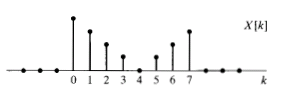
\includegraphics[scale=1]{p8-32-a.png} 

A new sequence $y[n]$ of length 16 is defined by 

\[y[n] = \begin{cases} x\left[ \frac{n}{2}\right], & n \text{ even}\\
0, & n \text{ odd} \end{cases} \]

Which plot corresponds to $Y[k]$, the 16-point DFT of $y[n]$?

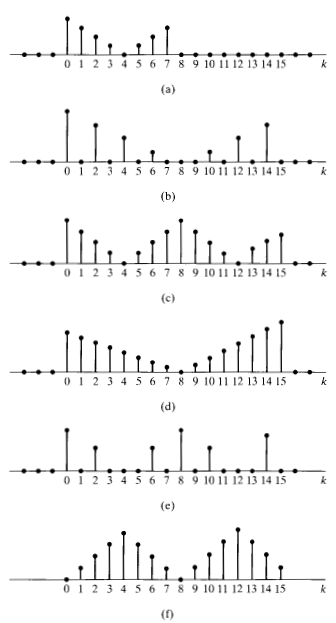
\includegraphics[scale=1]{p8-32.png} 

{\color{blue}
The DTFT of $y[n[$ is related to the DTFT of $x[n[$ as follows: 

$Y(\omega) = X(2\omega)$. The DFT is samples of the DTFT, so $X[k] = X(\omega)\big|_{\omega = \frac{2 \pi k}{N}}$ and $Y[k] =Y(\omega)\big|_{\omega = \frac{2 \pi k}{2N}} = X(2\omega) \big|_{\omega = \frac{2 \pi k}{2N}} = X(\omega) \big|_{\omega = \frac{2 \pi k}{N}}$. 

From the periodicity of the DTFT, we see that $Y[k] = \begin{cases}X[k], & k=-0,\ldots, N-1 \\ X[k-N], & k = N, \ldots, 2N-1\end{cases} = X[k \text{ mod } N] \text{ for } k=0,\ldots, 2N-1$
}


\section{DFT and the DTFT}
% 8.61 in the 3rd ed

Let $x[n]$ be real-valued and non-negative over $0\leq n \leq N-1$ and zero otherwise. Let $X[k]$ be the $N$-point DFT of $x[n]$ and $X(e^{j\omega})$ be the DTFT of $x[n]$.

\subsection*{True or false?}
If $X(e^{j\omega})$ can be written as 
\[X(e^{j\omega})=B(\omega)e^{j \alpha \omega}\]
where $B(\omega)$ is real and $\alpha$ is a real constant, then $X[k]$ can be expressed as \[X[k]=A[k]e^{j \gamma k}\]
where $A[k]$ is real and $\gamma$ is a real constant.

{ \color{blue}
True! 

Consider any signal $x[n]$ such that $X(e^{j\omega}) = B(\omega)e^{j\alpha \omega}$.
\begin{eqnarray*}
X[k] &=& X(e^{j\omega})\big|_{\frac{2 \pi k}{N}} \\ 
&=& B\left(\frac{2 \pi k}{N}\right)e^{j\frac{2 \pi}{N}k \alpha} \\
A[k] &=& B\left({\frac{2 \pi k}{N}}\right) \\
\gamma &=& \frac{2 \pi \alpha}{N}
\end{eqnarray*}
}

\subsection*{True or false?}
If $X[k]$ can be expressed as 
\[X[k]=A[k]e^{j \gamma k}\]
where $A[k]$ is real and $\gamma$ is a real constant, then $X(e^{j\omega})$ can be written as \[X(e^{j\omega})=B(\omega)e^{j \alpha \omega}\]
where $B(\omega)$ is real and $\alpha$ is a real constant.

{ \color{blue}
False!

Take as a counter example: $x[n] = \delta[n]+\frac{1}{2}\delta[n-1]$.

\[
X[k] = 1+\frac{1}{2}e^{-j\pi k} = 1+\frac{1}{2}(-1)^k
\]

which can be expressed as $X[k] = A[k] e^{j\gamma k}$ with $A[k] = 1+\frac{1}{2}(-1)^k$ and $\gamma = 0$.

However, the DTFT of $x[n]$ is $X(e^{j \omega}) = 1 + \frac{1}{2}e^{j\omega}$, which cannot be expressed as $X(e^{j\omega}) = B(\omega)e^{j\alpha\omega}$.

This makes sense because the DFT is samples of the DTFT, so knowing that the DTFT has linear phase means the DFT must have linear phase, but knowing the DFT has linear phase does not guarantee the DTFT has linear phase at unsampled points.
}

\section{Removing Distortion with the DFT}
% 8.67 in3rd ed

Let a distorted signal $y[n]$ be the output of an LTI system (defined by $h[n]$) on the true signal $x[n]$. Our goal is to recover $x[n]$ from $y[n]$ with knowledge of the filter $h[n]$. In theory, $x[n]$ can be recovered from $y[n]$ by passing $y[n]$ through an inverse filter having a system function equal to the reciprocal of the system function of the distorting filter.

Suppose that the distortion is caused by an FIR filter with impulse response 
\[ h[n] = \delta[n] -\frac{1}{2}\delta[n-n_0] \]
where $n_0$ is a positive integer, i.e. the distortion of $x[n]$ take sthe form of an echo at delay $n_0$.

\begin{description}
\item[(a)] Determine the z-transform $H(z)$ and the $N$-point DFT $H[k]$ of the impulse response $h[n]$. Assume that $N = 4n_0$.
\item[(b)] Let $H_i(z)$ denote the system inverse function of the inverse filter, and ler $h_i[n]$ be the corresponding impulse response. Determine $h_i[n]$. Is this an FIR or an IIR filter? What is the duration of $h_i[n]$?
\item[(c)] Suppose that we use an FIR filter of length $N$ in an attempt to implement the inverse filter, and let the $N$-point DFT of the FIR filter be
\[ G[k]=\frac{1}{H[k]}, \quad k=0,1,\ldots,N-1 \]
What is the impulse response $g[n]$ of the filter?
\item[(d)] It might appear that the FIR filter with DFT $G[k]=\frac{1}{H[k]}$ implements hte inverse filter perfectly. After all, one might argue that the FIR distorting filter has an $N$-point DFT $H[k]$ and the FIR filter in cascade has an $N$-point DFT $G[k]=\frac{1}{H[k]}$, and since $G[k]H[k]=1$ for all $k$, we have implemented an all-pass, nondistorting filter. What is the fallacy in this argument?
\item[(e)] Perform the convolution of $g[n]$ with $h[n]$, and thus determine how well the FIR filter with $N$-point DFT $G[k]=\frac{1}{H[k]}$ implements the inverse filter.
\end{description}

{\color{blue}
%\subsection*{(a)}
%The x-transform of $h[n]$ is 

%\subsection*{(b)}

%\subsection*{(c)}

%\subsection*{(d)}

Coming later...
}

\end{document}